\chapter{テーブルとレコードとアトリビュート}

SQLを学ぶために、まず、テーブルとレコードとアトリビュートは、どのようなものかを見ていくことにしましょう。前の章で、テーブルは丸、レコードはその丸の中のどこかにあるもの、という説明をしました。そして、アトリビューtについての説明ははしょりました。

この章では、この先SQLを学ぶのに必要なこととして、テーブルとレコードとアトリビュートについて、学び直していくことにします。


\section{テーブル}

リレーショナルデータベースのテーブルとは、どのようなものでしょうか。一言で言ってしまえば、レコードという要素がどこかに存在する空間です。レコードは、この空間の中のどこかにある要素となります。

テーブルが何であり、レコードはテーブルの中でどのように存在しているのでしょうか。

\subsection{レコードの位置}

テーブルの中で、レコードはどこにあるのでしょうか。テーブルという空間の中で、レコードがどこにあるかは、そのレコードのアトリビュートの値で決まります。詳細は後で説明しますが、アトリビュートが座標と考えることができます。

たとえば、整数のアトリビュートを一つだけ持つレコードが定義されているとします。このとき、レコードを、数直線上のその値に対応している馬謖尾置いたと考えます。そうすると、テーブルという空間は数直線の形をしていて、レコードの場所は、その数直線上のどこかという様に考えることができます。

\begin{table}[htb]
  \begin{tabular}{|c|} \hline
    number \\ \hline
    1 \\
    2 \\
    3 \\
    5 \\ 
    8 \\ \hline
  \end{tabular}
  \label{table:number}
  \caption{数字のテーブル}
\end{table}

\begin{figure}[htbp]
	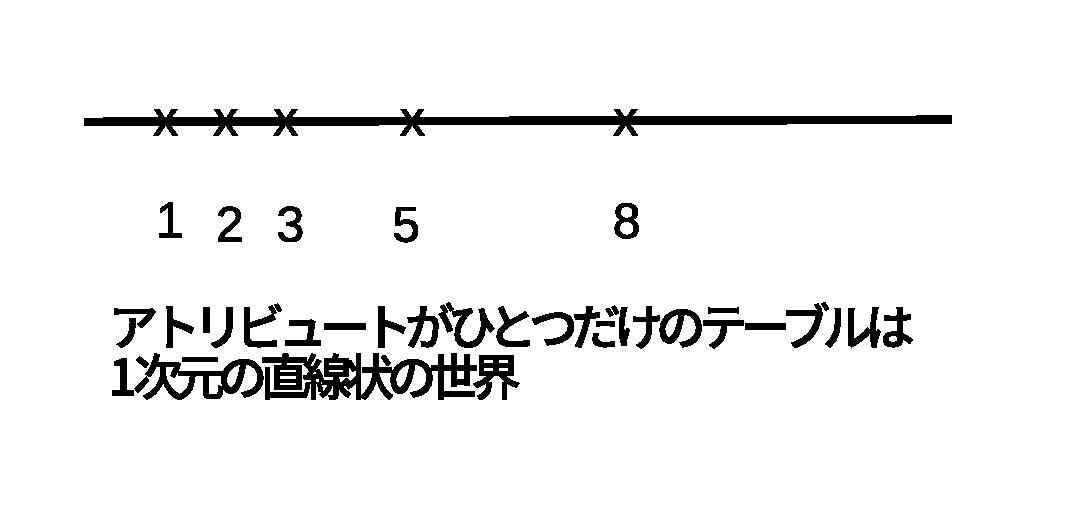
\includegraphics[width=12cm,clip]{draw/line.eps}
	\caption{アトリビュートがひとつのテーブルとレコード}
	\label{fig:line_like}
\end{figure}

\subsection{テーブルの中身には順番がない}


テーブルの中にはレコードがあるのですが、そのレコードにはなんらかの順番があるのでしょうか。結論から行けば、テーブルの中にあるレコードに、順番はありません。データベースに登録した順番や、特定のアトリビュートの値が順番になるのではありません。データベースのなかでは、レコードは順番が定義されません。

先程、たーブルという空間がが数直線で現せる例を出しました。ですが、その数直線上の場所は、順番wの現すものでは有りません。もう一度書くと、順番をあらわすものでは無く、場所をあらわすものでしかありません。

大切なことなのでもう一度言いますが、テーブルの中のレコードには、順番がありません。これは、読み出しを行ったとき、入れた順番や、プライマリキーの値の順番で結果が取り出せることを期待してはならない、ということです。
これは、limitを使ってひとつだけ要素を取り出す場合、特定のレコードが必ず取り出せることを期待してはならないということでもあります。

\subsection{順番はどうやってつけるのか}

ですが、SELECTにORDER BYとつけると、出てきた結果に何らかの順番を付けることができます。
では、ORDER BYで定義される順番はなんなのでしょうか。

それは、データベースから取り出すときにソーティングを行って、定義された順番で並べています。そのため、順番で取り出す必要が無いときは、ORDER BYを書かない方が読み出しは早くなります。



\section{レコードとアトリビュート}

今度はレコードとアトリ牛ーとを絵どう考えたらいいかを考えてみましょう。データベースの入門書では、レコードを伝票の1枚に例えたり、スプレッドシートの列二例えたりしていることが多くあります。ですが、リレーショナルデータベースを理解するためには、全く別のイメージをする必要があります。

\subsection{レコード}

\begin{figure}[htbp]
	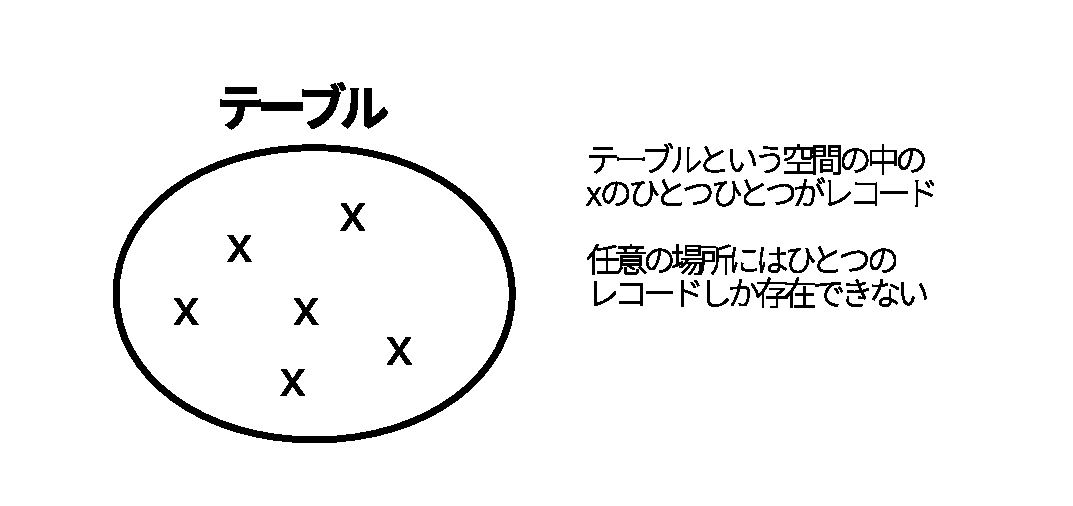
\includegraphics[width=12cm,clip]{draw/record.eps}
	\caption{テーブルとレコード}
	\label{fig:record}
\end{figure}

レコードとは、テーブルという空間のどこかにある要素です。どくにあるかという場所は、そのレコードが持っている情報、具体的には、アトリビュートの値によって決定されます。

レコードは、テーブルという空間のどこかにあります。このレコードは、テーブルの中にいくつあっても構いません。ですが、完全に同じ場所に、二つのレコードが存在することはできません。これは、レコードの全てのアトリビュートの値が同じであるレコードは同じものが存在すると、区別ができないということです。

\subsection{アトリビュートの役割と座標軸}

\begin{figure}[htbp]
	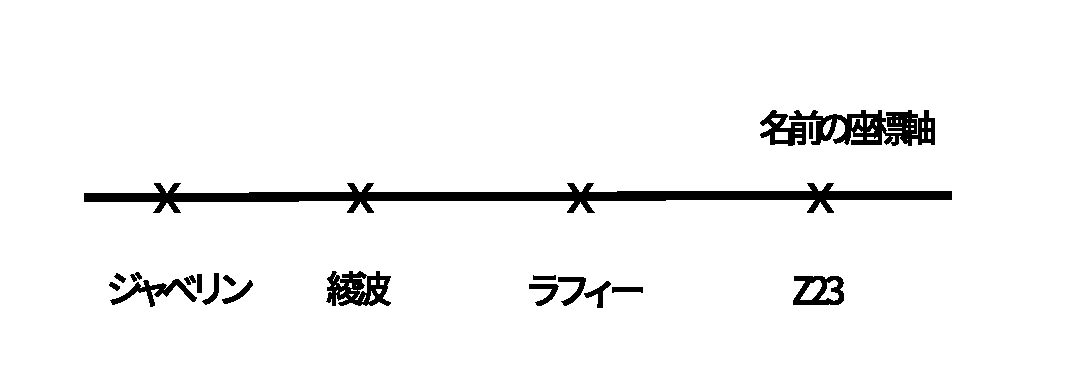
\includegraphics[width=12cm,clip]{draw/name_axis.eps}
	\caption{名前という座標軸}
	\label{fig:name_axis}
\end{figure}


ここまで、テーブルの中でレコードがどこにあるかは、アトリビュートによって決まる、という表現をしてきました。では、そのアトリビュートをどのように捉え直せば良いのでしょうか。

アトリビュートは、そのテーブルという空間の場所をあらわす、座標軸です。座標軸、というと、数字であらわ競れるものをイメージするかも知れません。ですが、これは、もっと広い意味での座標となります。

名前というアトリビュートをもつレコードと、そのレコードが存在するテーブルを考えましょう。このとき、テーブルは、名前、という座標軸で場所をあらわすことができる空間になります。名前、という座標軸は、無限にある全ての名前をに対応する場所を、全て座標として定義できるものとします。

\subsection{テーブルという多次元空間}

実際のレコードは、複数のアトリビュートを持ちます。つまり、座標軸が複数あります。これは、どのように考えるのが良いのでしょうか。

レコードのアトリビュートは、それぞれが独立して存在しています。たとえば、名前と所属、という二つのアトリビュイートがあったとして、この二つはお互いに、もう一方に影響を与えることはありません。
数学では、このような関係を、直交といいます。直交はJOINの時にも出てくる概念なので、ここではそういうものと覚えてください。

アトリビュートがテーブルの中の座標をあらわすことと、先程の直交という概念を組み合わせるとどうなるでしょうか。それは、テーブルの中のレコードの場所は、直交座標系で著わすことができるということになります。つまり、テーブルとは、1次元以上の次元を持った多次元の直交座標系であらわわされる空間です。

\subsection{1次元のテーブル}

レコードがひとつのアトリビュートのみをもつテーブルは、1本の座標軸でもある直線であらわされう空間上のどこかに、レコードがあるテーブルと考えることができます。これは、図\ref{fig:name_axis}のようにあらわされます。

何度も書きますが、この座標軸の上で、レコードがどこにあるかで順番は決まりません。アトリビュートが定義するのは、テーブルの上でレコードがある場所だけです。

\subsubsection{2次元のテーブル}

アトリビュートが二つのレコードをもつテーブルは、直交座標系の平面として考えることができます。先程の例で、名前と所属というアトリビュートをもつレコードを考えました。そのようなレコードを要素にもつテーブルは、名前という座標軸と所属という座標軸が直交する、直交座標系で表現できる平面です。

\begin{table}[htb]
  \begin{tabular}{|c|c|} \hline
    名前 & 所属 \\ \hline
    ジャベリン & ロイヤル \\
    綾波 & 重桜 \\
    ラフィー & ユニオン \\
    Z23 & 鉄血 \\ \hline
  \end{tabular}
  \label{table:names_belongs}
  \caption{名前と所属のテーブル}
\end{table}

表\ref{table:names_belongs}のレコードをもつテーブルで、それぞれのレコードがどこにあるかは、図\ref{fig:2daxis}の直交座標系であらわすことができます。

\begin{figure}[htbp]
	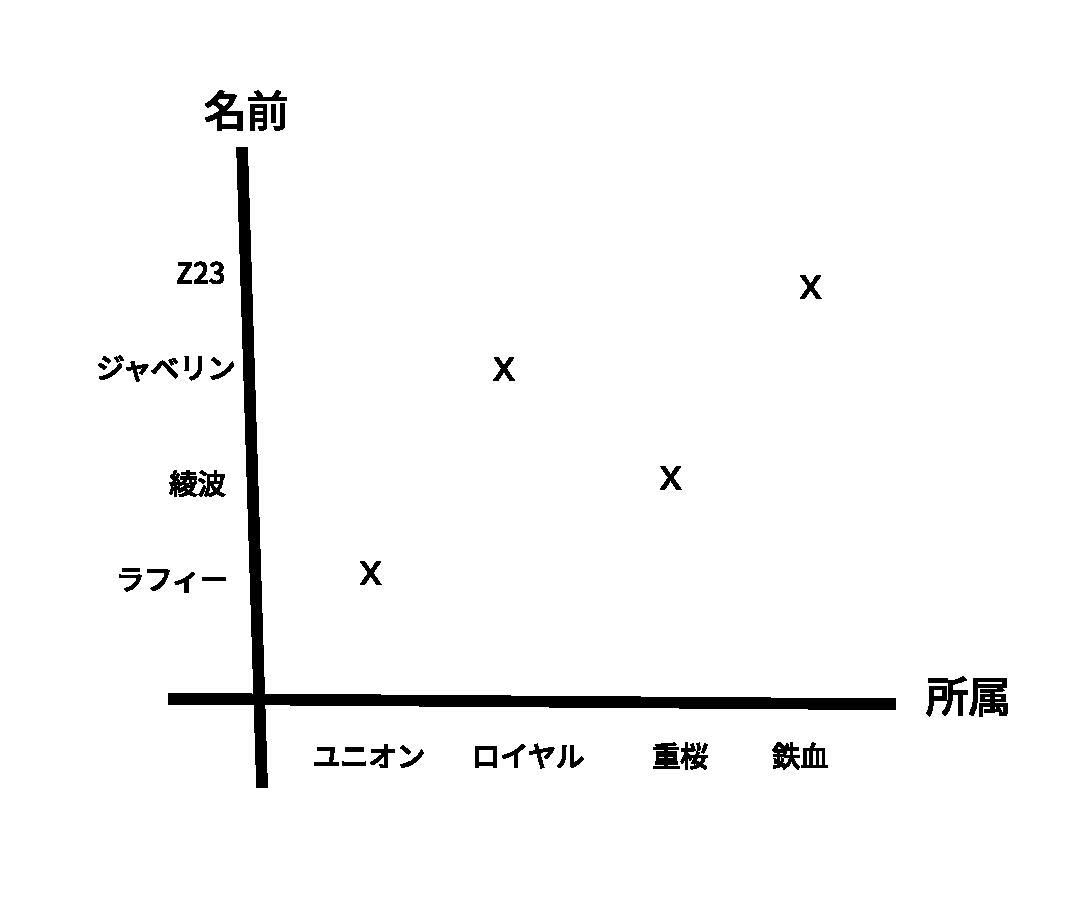
\includegraphics[width=12cm,clip]{draw/2daxis.eps}
	\caption{テーブルに対応した直交座標系}
	\label{fig:2daxis}
\end{figure}


この平面だと、アトリビュートはあくまでも座標であり、順番を表すものではない、とうのがよりイメージしやすいと思います。そして、SELECTで要素を選ぶというのは、ある座標軸の上にある要素をえらぶ、ということでもあります。厳密には違うのですが、今はそのようにイメージしてください。

\subsubsection{3次元のテーブル}

アトリビュートがみっつのレコードを持つテーブルを考えてみましょう。名前、所属、感種別、というみっつのアトリビュートを考えます。このレコーっどを要素としてもつテーブルは、3本の直交する座標軸で表現される、3次元空間になります。

\begin{figure}[htbp]
	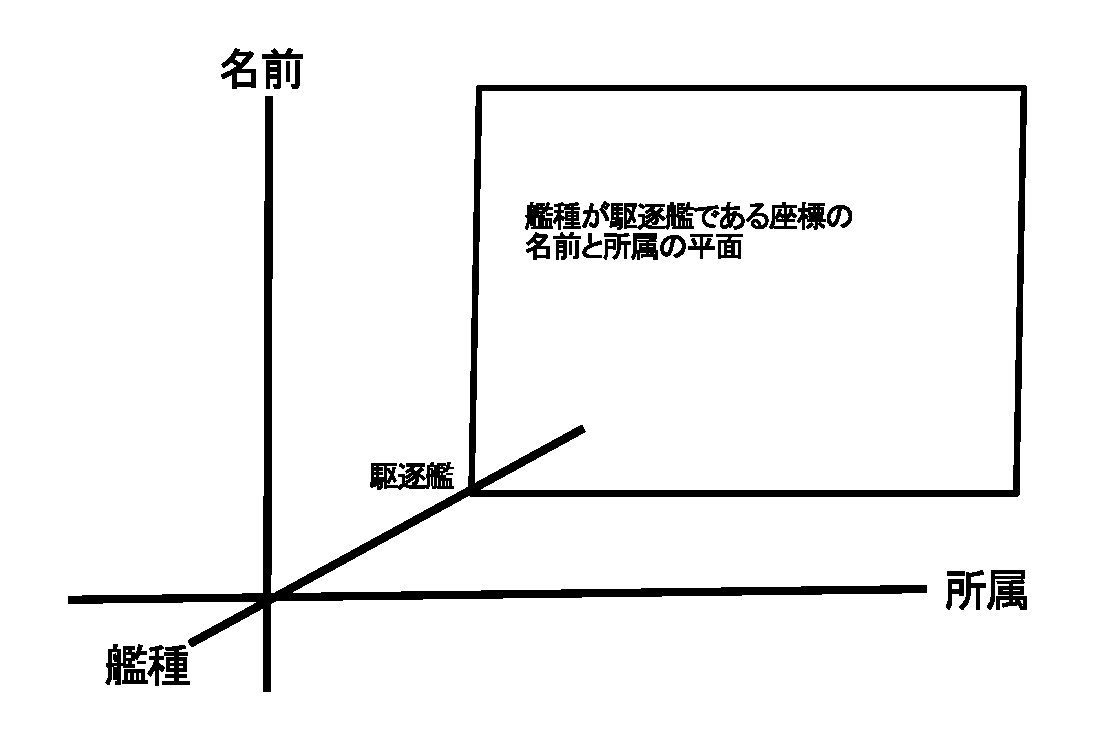
\includegraphics[width=12cm,clip]{draw/3daxis.eps}
	\caption{三次元のテーブルの直交座標系}
	\label{fig:3daxis}
\end{figure}

図\ref{fig:3daxis}のような座標系の中でSELECTをするとはどういうことかを考えてみましょう。それは、三次元空間として著わされるテーブルの中で、ある範囲にあるもの全てをとりだす、というような考え方になります。

\begin{verbatim}
SELECT 名前,所属 FROM ships
WHERE 艦種 = '駆逐艦' ;
\end{verbatim}

たとえば、このSELECTは、座標の艦種が駆逐艦である、全ての要素を取り出すということです。これは、座標の艦種が駆逐艦のところにある、座標名前と座標の所属であらわわされる、平面上にある要素を全て取り出すというように考えることができます。

\subsubsection{4次元以上のテーブル}

アトリビュートの数が四つ胃異常のレコードをもつテーブルは、4次元以上の、多次元の空間です。例えば、アトリビュートをよっつ持つレコードのテーブルは、お互いに直交する座標軸が4本で著わされる空間となります。
4次元以上はイメージがしにくいかも知れませんが、実際のテーグルは、直交作法で著わされることに変わりはありません。それが、多次元となっているだけです。

